\subsection{Seam allowance}

Seam allowance is crucial to the construction of a backpack. After experimenting a lot, I realised I tend to sew seams 10mm to 15mm from the side of the fabric. With that in mind, if I leave more than 15mm of fabric for the seem allowance - say 30mm - I would make a mess of my well thought pack dimensions because every seam would add overall 30mm extra fabric for each bond. That will end up in a much bigger pack than originally designed, and you definitely want to avoid that. I have ended up with a couple of backpacks that just look weird because of messed up dimensions.

It's also the perfect allowance for binding the seams at a later stage.

\begin{figure}[H]
  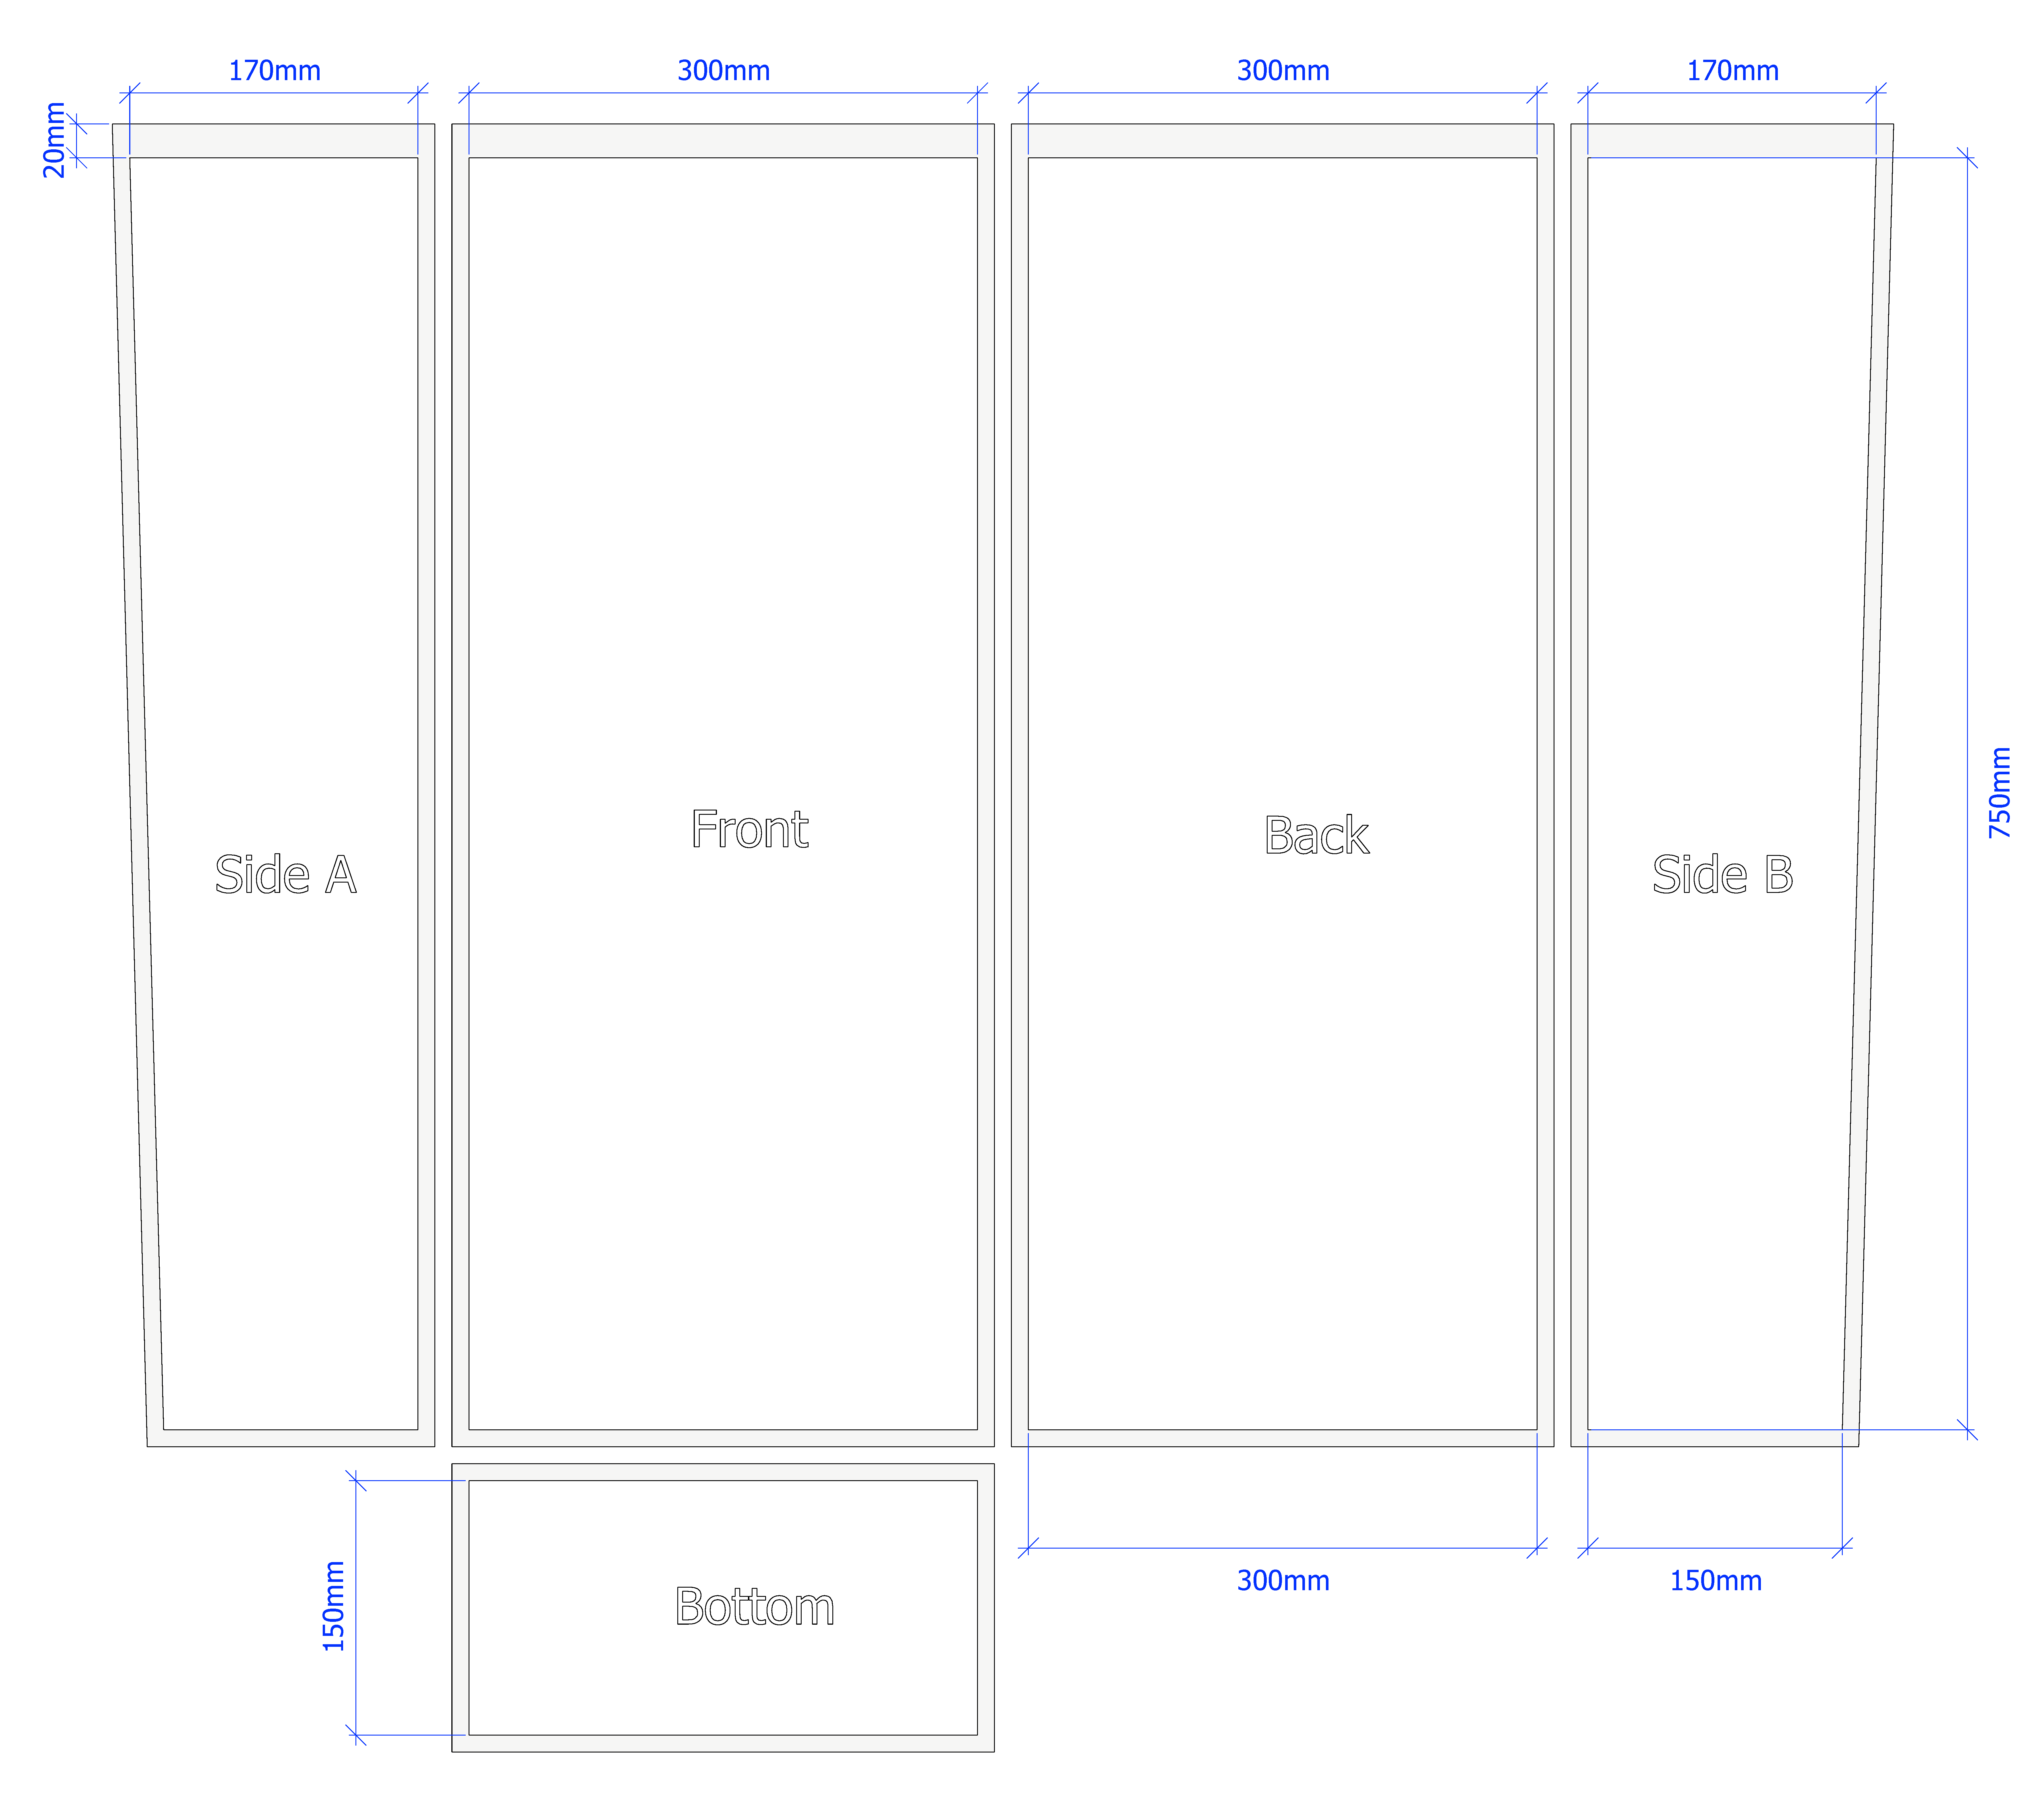
\includegraphics[width=\textwidth]{media/sketches/pack-rough-cut}
  \caption{Rough backpack dimensions including seam allowance of 15mm}
  \label{img:gear-database}
\end{figure}
